\documentclass[conference]{IEEEtran}

\usepackage[utf8]{inputenc}
\usepackage[T1]{fontenc}
\usepackage{amsmath,amssymb,amsfonts,amsthm,mathtools}
\usepackage{graphicx}
\usepackage{tikz}
\usetikzlibrary{arrows.meta,positioning,fit,backgrounds}
\usepackage{booktabs}
\usepackage{multirow}
\usepackage{array}
\usepackage{xcolor}
\usepackage{url}
\usepackage{cite}
\usepackage{algorithm}
\usepackage{algorithmic}
\usepackage[colorlinks=true,linkcolor=black,citecolor=black,urlcolor=black]{hyperref}
\usepackage{orcidlink}

\graphicspath{{figures/}}

\theoremstyle{definition}
\newtheorem{definition}{Definition}
\newtheorem{assumption}{Assumption}
\newtheorem{proposition}{Proposition}
\theoremstyle{remark}
\newtheorem{remark}{Remark}

% Shared notation for Workload-Compiled Retrieval.
\newcommand{\R}{\mathbb{R}}
\newcommand{\E}{\mathbb{E}}
\newcommand{\Q}{\mathcal{Q}}
\newcommand{\A}{\mathcal{A}}
\newcommand{\W}{\mathcal{W}}
\newcommand{\C}{\mathcal{C}}
\newcommand{\D}{\mathcal{D}}
\newcommand{\B}{\mathcal{B}}
\newcommand{\F}{\mathcal{F}}
\newcommand{\WCR}{\textsc{WCR}}
\newcommand{\CWC}{\textsc{CWC}}
\newcommand{\Rcert}{R^{\mathrm{cert}}}
\newcommand{\q}{q}
\newcommand{\cell}{c}
\newcommand{\plan}{a}
\newcommand{\features}{x}
\newcommand{\utility}{u}
\newcommand{\latency}{\ell}
\newcommand{\score}{s}
\DeclareMathOperator*{\argmax}{arg\,max}
\DeclareMathOperator*{\argmin}{arg\,min}

% Run-in heading: IEEEtran numbers \paragraph as ``a)'', which produced a stray
% enumerator at the head of the results section (R1-D9) and buried a run-in heading
% inside a paragraph (R1-D13).
\newcommand{\parhead}[1]{\par\smallskip\noindent\textbf{#1}\ }

\IEEEoverridecommandlockouts
\title{Certified Workload-Window Plan Selection for Hybrid Vector Search under SLOs}

\author{%
\IEEEauthorblockN{%
Yanxiao~Li\textsuperscript{1}\,\orcidlink{0009-0008-3389-1619},
Junhao~Wei\textsuperscript{1}\,\orcidlink{0009-0006-0553-2032},
Yifu~Zhao\textsuperscript{1}\,\orcidlink{0009-0004-2363-9269},
Haochen~Li\textsuperscript{1}\,\orcidlink{0009-0000-8213-5854},
Xu~Yang\textsuperscript{1}\,\orcidlink{0000-0002-7037-3609},
Sio-Kei~Im\textsuperscript{2}\,\orcidlink{0000-0002-5599-4300},
Yapeng~Wang\textsuperscript{1,*}\,\orcidlink{0000-0002-1085-5091}}
\IEEEauthorblockA{%
\textsuperscript{1}Faculty of Applied Sciences, Macao Polytechnic University, Macao SAR, China\\
\textsuperscript{2}Macao Polytechnic University, Macao SAR, China\\
\textsuperscript{*}Corresponding author: Yapeng Wang (e-mail: yapengwang@mpu.edu.mo)}
\thanks{This work was supported by the FDCT--MOST grant 0018/2025/AMJ and by Macao Polytechnic University grant RP/FCA-25/2025. Manuscript submitted June~2026.}}
\date{}

\begin{document}

\maketitle

\begin{abstract}
Hybrid vector search engines expose many physical plans---lexical retrieval, dense retrieval, learned-sparse retrieval, late interaction, fusion, metadata filtering, and reranking. Selecting a plan under a latency SLO is a query-optimization problem, yet static policies and per-query routers give little assurance that the chosen plan stays feasible once the next workload window shifts. We propose \CWC{}, a certified workload-window compiler for hybrid-search plan selection. Given a labeled historical workload, an unlabeled incoming workload window, and telemetry from candidate operators, \CWC{} partitions queries into workload cells, binds each cell to a physical plan, and abstains to a feasibility-best fallback when the selected plan is fragile. Its certificate is a finite-sample, distribution-free upper bound on the evaluation-window SLO-violation rate under a specified within-cell shift budget; in experiments, a conservative plug-in budget upper-bounds the realized violation in every run. On a $45$-block study over SciFact, FiQA, and NFCorpus with BM25, E5, Qwen3-Embedding, SPLADE, ColBERTv2, fusion, and reranking actions, \CWC{} ranks first on constrained utility, significantly outperforms four strong static operators, and statistically ties calibration-aware selectors while adding a deployment certificate they lack. At the binding budget it cuts realized SLO violations from about $11\%$ to about $0.1\%$ at roughly $4\%$ nDCG cost, and a scaling study shows the certified bound tightens with per-cell calibration size, as the theory predicts.

\end{abstract}

\begin{IEEEkeywords}
Hybrid search, vector search, query processing and optimization, physical plan selection, workload-aware optimization, service-level objectives, distribution-free risk control
\end{IEEEkeywords}

\section{Introduction}
\label{sec:introduction}

Modern data systems increasingly embed hybrid and vector search. Production hybrid-search stacks combine BM25~\cite{robertson2009bm25}, dense vector search~\cite{wang2022e5}, learned-sparse retrieval~\cite{formal2021splade}, late interaction~\cite{santhanam2021colbertv2}, reciprocal-rank fusion~\cite{cormack2009rrf}, metadata-filter placement, and neural reranking~\cite{pradeep2023rankzephyr}. This is the operator menu that the retrieval literature and current vector engines expose in general; we do not model one particular deployment, and the action catalog we actually execute is listed in Table~\ref{tab:catalog}. These are \emph{physical plans} with different latency profiles, filter behavior, and failure modes, so the systems question is a query-optimization one: which physical plan should serve a workload under a latency SLO and a filter constraint, and, critically, can that choice be \emph{trusted} once the workload drifts from what was seen at calibration. A plan that is fast on yesterday's queries can silently start violating the latency SLO when today's workload shifts toward harder, higher-selectivity queries. In deployment the quantity that matters is the \emph{rate} at which the chosen plan breaches the SLO over a serving window: this rate drives SLA penalties and admission decisions, yet current selectors set it by hoping a plan generalizes, with no guarantee before execution. Bounding it ahead of time---so an operator can audit, and admit or hold back, a plan before it serves traffic---is the gap we close.

Most current strategies choose at the wrong unit and offer no such trust. Fixed recipes such as BM25-only, dense-only, fixed fusion, or fixed reranking depth are simple but brittle: the best plan changes with selectivity, budget, and query mix. Per-query routers are more adaptive, but they decide from isolated query features, and the documented unreliability of query performance prediction makes per-query selection fragile in exactly the constrained regime we care about. Neither family, however, says anything about \emph{how often the deployed choice will violate the SLO on the next, possibly shifted, workload window}. An arriving workload window, however, can be observed before execution: it reveals stable regions where the same plan is repeatedly good, and it lets a system bound its own risk instead of merely hoping the chosen plan generalizes.

This paper treats hybrid-search plan selection as \emph{workload-window physical-plan compilation with an auditable deployment guarantee}. The input is a labeled training workload, an unlabeled evaluation workload window, and telemetry from candidate operators; the output is a compiled design---queries partitioned into plan cells, a physical plan bound to each cell, a cell-level plan frontier---together with a \emph{distribution-free, finite-sample certificate} on the eval-window SLO-violation rate that holds under a bounded amount of workload shift. The certificate is operational: when a cell's plan is not certifiably safe, the compiler abstains to a certifiably feasible fallback. The operators themselves are unchanged; what is new is that the optimizer certifies \emph{which plan to deploy, and when to abstain}, the way a database physical-design tool reasons about a workload rather than a single query. To our knowledge no prior hybrid-search method provides such a guarantee, and none of our baselines provides one as used.

Our system is \CWC{}, the \emph{Certified Workload-window Compiler}. \CWC{} first embeds train and evaluation queries using observable workload telemetry---cheap retrieval probes, score-shape features, branch overlap, filter survival, and latency signals---then partitions the workload into plan cells and binds each cell to the action with the best training constrained utility, so each evaluation query inherits the plan of its cell. On top of this it adds an abstain rule and a deployment certificate, both developed later in the paper. We write \WCR{} for the \emph{un-guarded} variant (the same compiler without the abstain rule); it is used only as an ablation and in the preliminary single-collection pilot and cross-dataset audit, and when no cell abstains \CWC{}$\equiv$\WCR{}. The method is transductive in the systems sense: it uses unlabeled telemetry from the current workload window, but never evaluation relevance labels.

Our canonical evidence (Section~\ref{sec:results-rank}) is a $45$-block study over SciFact, FiQA, and NFCorpus with real external operators under a controlled bounded workload shift; a single-collection NFCorpus pilot and a $360$-block cross-dataset audit corroborate it as robustness, not the headline.

The claim is intentionally scoped: optimizer-level gains plus an auditable deployment guarantee under a fixed action catalog, not universal superiority over every retriever stack. In particular \CWC{} \emph{ties} the strongest calibration-aware selectors on mean utility; its differentiator there is the certificate, not raw rank.

This paper makes three contributions.
\begin{enumerate}
  \item \textbf{Abstraction.} We formulate hybrid-search plan selection as \emph{certified workload-window physical-plan compilation}: an unlabeled workload window is partitioned into plan cells, each cell is bound to an executable physical plan, and each deployment decision carries an auditable risk guarantee.
  \item \textbf{Guarantee.} We prove a distribution-free, finite-sample certificate (Proposition~\ref{prop:cert}) that upper-bounds the eval-window SLO-violation rate under a bounded within-cell shift budget, made operational through \CWC{}, a guarded compiler that abstains to a feasibility-best fallback on fragile cells; a density-ratio upper-confidence-bound variant removes the assumed-shift caveat. To our knowledge this is the first such guarantee at the \emph{workload-window} granularity for hybrid-search plan selection.
  \item \textbf{Evaluation.} On a $45$-block SciFact+FiQA+NFCorpus workload with BM25, E5, Qwen3-Embedding, SPLADE, ColBERTv2, fusion, and reranking actions, \CWC{} is average-rank first on constrained utility, Holm-beats four strong static operators, and ties calibration-aware selectors while adding a certificate they lack, cutting realized SLO violations from $\approx11\%$ to $\approx0.1\%$ at $\approx4\%$ nDCG cost; under an SLA admission-control objective it separates from those selectors (rank $1.44$, Holm-beating all six baselines), and a scaling study confirms the bound tightens with per-cell calibration size. Ablations and a $360$-block audit isolate the source of the gains.
\end{enumerate}

\section{Related Work}
\label{sec:related}

One framing prevents most confusion with prior art: we do not propose another retriever, reranker, or fusion rule, and our gains do not come from a stronger embedding model. We certify a \emph{deployment decision}---which existing physical plan to run for a workload window, and when to abstain---under a distribution-free guarantee. Read this way, the closest neighbors fall into four groups, and \CWC{} differs from each in object or granularity rather than in the retrievers it uses: database query/physical-design optimization (different operator substrate and no risk guarantee), per-query routing and selective processing (per-instance, no workload-window guarantee), risk control / conformal methods (per-instance prediction sets rather than a certified plan choice under shift), and hybrid-retrieval operators and benchmarks (the actions we select among, not selectors themselves).

\parhead{Database query optimization.}
Classical query optimizers choose physical access paths and operator orders from a cost model (System R's cost-based access-path selection \cite{selinger1979accesspath}, Volcano's extensible search \cite{graefe1993volcano}), physical-design tools recommend indexes from workload-level what-if analysis \cite{chaudhuri1998autoadmin}, and adaptive systems such as Eddies re-route during execution under runtime shifts \cite{avnur2000eddies}. \WCR{} follows this tradition but changes the operator substrate: the physical actions are hybrid retrieval plans, not relational joins or scans, and the signals are retrieval telemetry rather than only cardinality estimates.

\parhead{Workload-level and transductive query optimization.}
A recent line of database work optimizes plans at the level of a workload rather than a single query. \textsc{LimeQO} casts offline query optimization as low-rank learning over a workload, exploiting structure shared across queries \cite{limeqo2025}, and Bayesian-optimization planners learn offline plans for repeated workloads \cite{bayesqo2025}. \WCR{} shares this workload-level, transductive stance but on a different substrate (hybrid-retrieval physical plans, not relational latency) and, unlike these methods, attaches a finite-sample guarantee that remains valid under bounded workload shift. On the retrieval side, \textsc{SearchGym} proposes a compositional configuration algebra for hybrid-search orchestration \cite{searchgym2026}; that work is a benchmarking and reproducibility substrate, whereas \WCR{} is an optimizer that \emph{selects and certifies} plans over such a space under constraints.

\parhead{Risk control and selective processing for retrieval.}
Conformal risk control gives distribution-free guarantees, and recent work applies it to ranked retrieval: two-stage conformal risk control bounds retrieval and ranking risk for a single ranker's output set \cite{angelopoulos2024twostagecrc}, while selective conformal risk control first selects confident instances and then applies conformal control \cite{xu2025selectiveCRC}. Per-query selective processing chooses a search configuration per request, often using query performance prediction, but a recent study shows these per-query gains are small and unreliable across collections \cite{qpplimits2025,selectiveqp2024}. Our certificate differs in granularity and object: it controls the \emph{eval-window} violation rate of a deployed per-cell plan under covariate/workload shift, exploiting the exactly observed cell masses, rather than constructing a per-instance prediction set. This window-level framing is also what lets us avoid the per-query unreliability documented in \cite{qpplimits2025}.

\parhead{Certified plan verification (the closest prior work).}
The nearest neighbor is CP4LQO~\cite{cp4lqo2025}, which makes learned \emph{relational} query plans verifiable by using conformal prediction to bound each plan's \emph{per-query latency} before execution, with adaptive-CP handling of distribution shift and a plan search guided by those bounds. We share its goal---a deployable guarantee on a learned plan choice under shift---but differ on three axes that are important to take into account. \emph{Object:} CP4LQO certifies a per-query latency interval; we certify a \emph{workload-window SLO-violation rate} $R_Q$, the aggregate quantity an SLA or admission controller actually needs, where per-query risk does not accumulate over the window. \emph{Granularity:} CP4LQO reasons per query, so its statistical risk grows with the number of queries; we partition the window into $K$ cells and, because the eval-window cell masses $m_\cell/M$ are observed exactly (transductive), only the $K$ within-cell expectations carry statistical risk and the mass term is estimation-error-free. \emph{Domain and operation:} CP4LQO targets relational SQL and guides plan \emph{construction}; we target constrained \emph{hybrid retrieval} (BM25/dense/SPLADE/ColBERTv2/fusion/rerank) and make the certificate operational through abstention to a selection-split feasibility-best fallback. Table~\ref{tab:certtax} places both in a small design space. We position our contribution as a workload-window certified \emph{compiler} for hybrid retrieval, not a new conformal-prediction technique.

\begin{table}[t]
\centering
\caption{Design space of certified plan selection under shift. Existing certified-plan work bounds per-query latency for relational SQL; \CWC{} occupies the workload-window violation-rate cell for hybrid retrieval.}
\label{tab:certtax}
\footnotesize
\resizebox{\columnwidth}{!}{%
\begin{tabular}{lll}
\toprule
 & \textbf{Per-query latency interval} & \textbf{Window violation-rate} \\
\midrule
Relational SQL & CP4LQO~\cite{cp4lqo2025} & --- \\
Hybrid retrieval & (per-query CP, unreliable~\cite{qpplimits2025}) & \textbf{\CWC{} (ours)} \\
\bottomrule
\end{tabular}}
\end{table}

\parhead{Learned query optimization, routing, and policy selection.}
Learning-augmented optimizers such as Bao steer query optimization while integrating with existing engines \cite{marcus2021bao}, and per-query routing / offline policy selection (e.g.\ contextual-bandit action selection with offline evaluation \cite{li2010contextualbandit}) choose an action per request from request-local features or logged rewards. \WCR{} learns plan choices from prior executions like these, and we use query-only and scalar-telemetry routers as baselines, but its unit of generalization is a workload cell in retrieval-telemetry space: it observes an unlabeled window, builds reusable cells, and returns a plan frontier and risk report rather than a per-instance relational-cost prediction or contextual classification.

\parhead{Hybrid-retrieval operators, reranking, and benchmarks.}
The actions we select among are standard hybrid-retrieval operators: BM25 \cite{robertson2009bm25}, dense (E5 \cite{wang2022e5}, BGE-M3 \cite{chen2024m3embedding}, Qwen3-Embedding \cite{zhang2025qwen3embedding}, NV-Embed \cite{lee2024nvembed}), learned-sparse SPLADE \cite{formal2021splade}, late-interaction ColBERT/ColBERTv2 \cite{khattab2020colbert,santhanam2021colbertv2}, reciprocal-rank fusion \cite{cormack2009rrf}, and neural rerankers such as RankZephyr \cite{pradeep2023rankzephyr}, which trade quality for latency. \WCR{} treats each as a physical action that may or may not be chosen for a cell, rather than proposing a new operator. Finally, the BEIR benchmark systematized the zero-shot evaluation of retrieval models \cite{thakur2021beir}; its metrics, however, score ranking quality alone and say nothing about deployability under a latency SLO; we evaluate constrained score, satisfaction, latency, regret, and rank-gated comparisons so quality and systems feasibility are tested together.

\section{Problem and Optimizer Model}
\label{sec:problem}

Hybrid retrieval exposes a catalog of executable physical actions rather than a single scoring function. \emph{On the word ``telemetry''.} We use it for everything the optimizer may read \emph{before} committing a plan for the incoming window, which is of two kinds: (i) quantities computed or estimated up front for the query at hand---query-derived features, filter-survival estimates, and cheap retrieval-probe outputs; and (ii) quantities genuinely observed from execution, such as latency, which are available for the labeled historical window but never for the window being compiled. Compiling the incoming window uses (i) on that window plus (i)--(ii) on history; no measurement of the incoming window's own execution is ever used. \emph{Notation:} $\W_{\mathrm{tr}},\W_{\mathrm{ev}}$ are the training and (unlabeled) evaluation workload windows; $\A$ the finite catalog of physical actions; $\features(\q,\W)$ the observable telemetry for query $\q$ computed in the context of the window $\W\in\{\W_{\mathrm{tr}},\W_{\mathrm{ev}}\}$ that contains it (the window enters only through window-level statistics such as filter survival and catalog state); $B,F$ the latency budget and metadata-filter setting; $\score$, $\latency$, and $\utility(\q,\plan;B,F)$ the ranking score, latency, and constrained utility of action $\plan$; and $\C,\gamma,\pi$ and $\D_{\W}$ the cell partition, assignment map, cell-plan binding, and compiled workload design.

Let $\W_{\mathrm{tr}}=\{\q_i\}_{i=1}^{n_{\mathrm{tr}}}$ be a labeled training workload and let $\W_{\mathrm{ev}}=\{\q_i\}_{i=1}^{n_{\mathrm{ev}}}$ be an unlabeled evaluation workload window. Let $\A$ be a finite catalog of physical actions. An action $\plan\in\A$ may be BM25 with pre-filtering, BM25 with post-filtering, a dense vector plan, reciprocal-rank fusion, an imported external ranking, or a reranking-depth plan. We use ``physical action'' consistently for these executable plans.

Each query has an observable telemetry vector $\features(\q,\W)\in\R^d$. Telemetry can include query-derived features, cheap retrieval-probe statistics, branch overlap, score concentration, filter survival estimates, and latency observations. Evaluation relevance labels are not observable when compiling $\W_{\mathrm{ev}}$.

\begin{definition}[Constrained utility and feasibility]
For query $\q$, action $\plan$, latency budget $B$, filter setting $F$, and penalty $\lambda>0$, the constrained utility is
\begin{equation}
  \utility(\q,\plan;B,F)=
  \score(\q,\plan;F)-\lambda[\latency(\q,\plan;F)-B]_+,
\end{equation}
where $[z]_+=\max\{0,z\}$. The feasibility indicator is
\begin{equation}
  \mathrm{feas}(\q,\plan;B,F)=\mathbf{1}\{\latency(\q,\plan;F)\le B\}.
\end{equation}
\end{definition}

For an evaluated set $S$ and policy $\rho:S\rightarrow\A$, satisfaction and regret are
\begin{align}
  \mathrm{Sat}(S,\rho)&=\frac{1}{|S|}\sum_{\q\in S}\mathrm{feas}(\q,\rho(\q);B,F),\\
  \mathrm{Reg}(S,\rho)&=\frac{1}{|S|}\sum_{\q\in S}
  \left[\max_{\plan\in\A}\utility(\q,\plan;B,F)-\utility(\q,\rho(\q);B,F)\right].
\end{align}
These metrics separate systems feasibility from ranking quality: a policy cannot be considered successful if it wins only by violating the latency budget.

\begin{definition}[Workload compilation]
A workload compiler chooses a partition $\C=\{\cell_1,\ldots,\cell_K\}$ of $\W_{\mathrm{tr}}\cup\W_{\mathrm{ev}}$, an assignment map $\gamma(\q)\in\{1,\ldots,K\}$, and a binding $\pi:\C\rightarrow\A$. The deployed policy for an evaluation query is
\begin{equation}
  \rho_{\C,\pi}(\q)=\pi(\cell_{\gamma(\q)}),\qquad \q\in\W_{\mathrm{ev}}.
\end{equation}
\end{definition}

The compiler may use relevance labels from $\W_{\mathrm{tr}}$ to bind actions, but it may use only telemetry from $\W_{\mathrm{ev}}$ when assigning evaluation queries to cells. For a fixed partition, the empirical binding objective is
\begin{equation}
\label{eq:cell-binding}
  \pi^\star(\cell)=
  \argmax_{\plan\in\A}
  \sum_{\q\in\cell\cap\W_{\mathrm{tr}}}
  \utility(\q,\plan;B,F).
\end{equation}
If a cell contains no training queries, the implementation falls back to the globally best training action under the same utility.

\begin{definition}[Compiled workload design]
The compiler returns
\begin{equation}
  \D_{\W}=(\C,\mathcal{P},\mathcal{R},\mathcal{G}).
\end{equation}
Here $\C$ is the workload-cell partition. $\mathcal{P}$ records, for each cell, the empirical plan frontier over ranking score, latency, and constrained utility. $\mathcal{R}$ records the estimated response of alternative actions in the cell. $\mathcal{G}$ records empirical stability statistics such as plan margin, bootstrap support, and risk flags (distinct from the distribution-free certificate of Section~\ref{sec:certificate}).
\end{definition}

\begin{assumption}[Workload-window observability]
The system observes $\W_{\mathrm{ev}}$ and can compute telemetry $\features(\q,\W_{\mathrm{tr}}\cup\W_{\mathrm{ev}})$ before final plan execution. It does not observe evaluation relevance labels during compilation.
\end{assumption}

\begin{proposition}[Cell-wise empirical optimality]
\label{prop:cell-optimality}
For any fixed partition $\C$ and any cell $\cell$ with at least one training query, the binding rule in Eq.~\eqref{eq:cell-binding} maximizes empirical constrained utility among all policies that assign one constant action to every training query in $\cell$.
\end{proposition}

\begin{proof}
For fixed $\C$ and $\cell$, a cell-constant policy is fully determined by its chosen action $\plan\in\A$. Eq.~\eqref{eq:cell-binding} enumerates the finite action catalog and selects the action with the largest empirical utility sum on $\cell\cap\W_{\mathrm{tr}}$. No other cell-constant action can have a larger empirical objective value by definition of the argmax.
\end{proof}

This proposition is intentionally modest. It does not claim optimality over all possible partitions or future workloads. It states the optimizer invariant used by \WCR{} once a workload partition is fixed. The empirical question in the rest of the paper is whether a telemetry-derived partition gives useful cell-constant physical designs under the constrained objective.

\section{\CWC{}: Workload-Window Plan Compiler}
\label{sec:optimizer}

This section describes the compiler core of \CWC{} (its un-guarded form \WCR{}); Section~\ref{sec:certificate} adds the abstain rule and certificate that complete \CWC{}. It is deliberately simple: the paper tests whether workload-level physical-plan compilation carries signal, not whether a complex controller can overfit a small benchmark. The implementation has four stages, shown in Figure~\ref{fig:framework}: construct an action catalog, compute workload telemetry, partition the workload, and bind/certify cell actions.

\begin{figure*}[t]
  \centering
  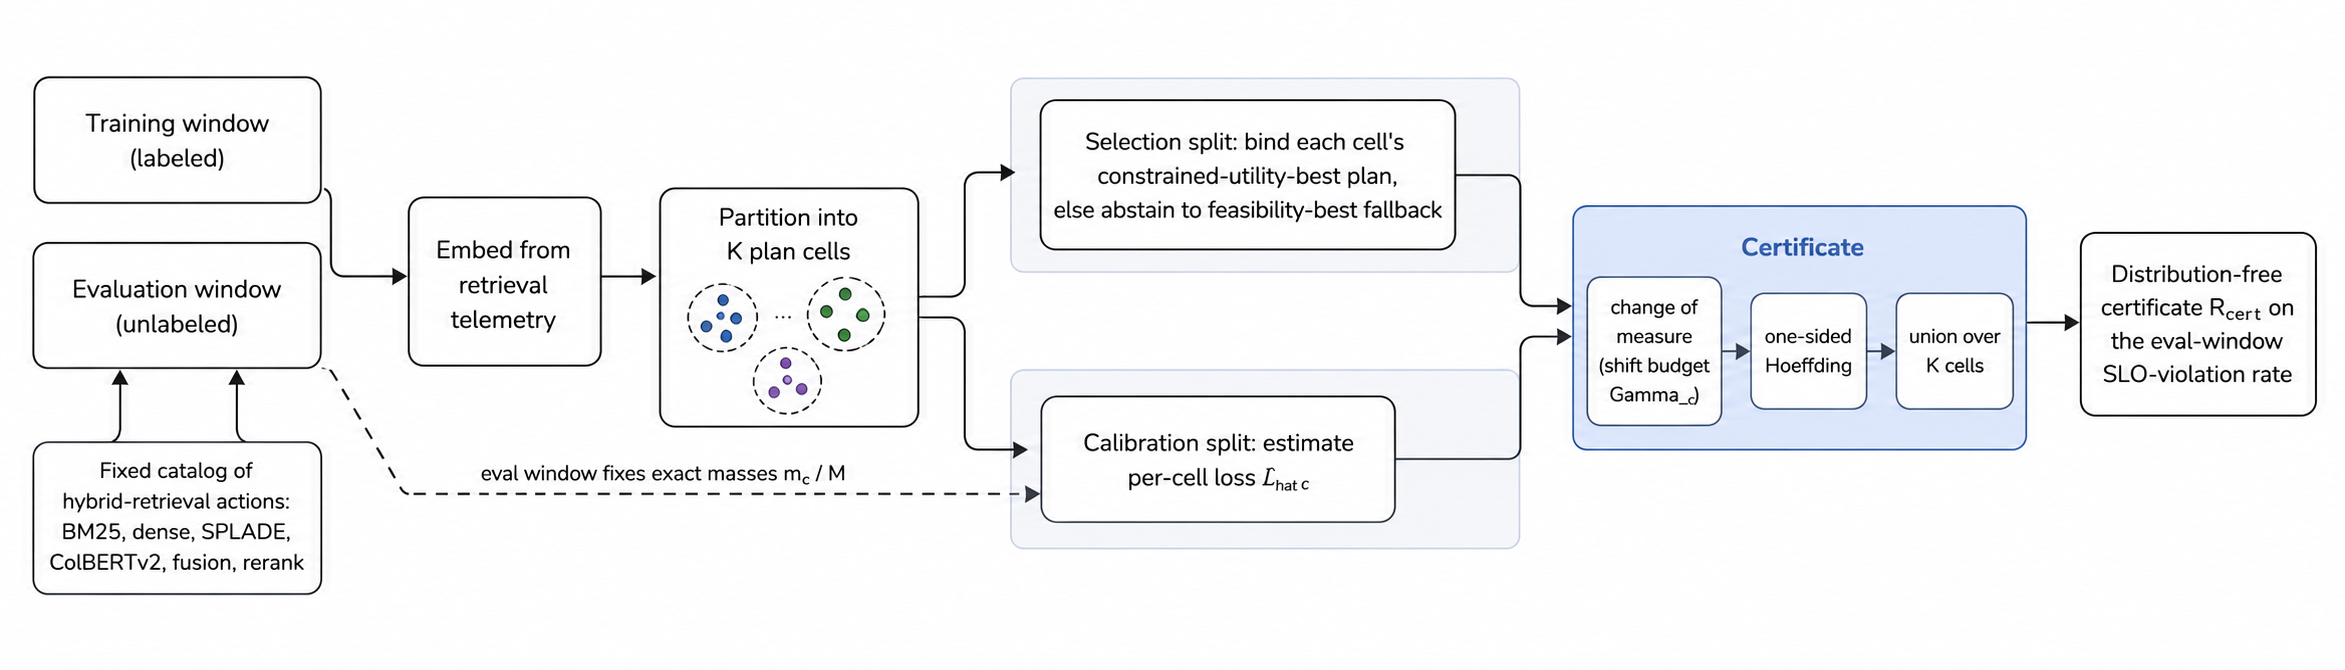
\includegraphics[width=0.95\textwidth]{cwc_framework}
  \caption{The \CWC{} pipeline. An unlabeled evaluation window and a labeled training window over a fixed action catalog are embedded into $K$ plan cells; the \emph{selection} split binds each cell's plan (or abstains to a feasibility-best fallback), the \emph{calibration} split estimates $\hat L_\cell$, and the eval window fixes the masses $m_\cell/M$. A change of measure under $\Gamma_\cell$ with one-sided Hoeffding and a union over $K$ cells gives the distribution-free certificate $\Rcert$ on the eval-window SLO-violation rate.}
  \label{fig:framework}
\end{figure*}

\subsection{Physical Action Catalog and Telemetry}

The action catalog treats retrieval systems as executable physical actions. In the main external-operator gate, $\A$ includes BM25 pre-filtering and post-filtering, dense retrieval, E5-base dense retrieval \cite{wang2022e5}, reciprocal-rank fusion \cite{cormack2009rrf}, weighted fusion, rerank depth 20, and external rankings imported from SPLADE \cite{formal2021splade}, ColBERTv2 \cite{santhanam2021colbertv2}, and Qwen3-Embedding-0.6B \cite{zhang2025qwen3embedding}. Static use of each action is also evaluated as a baseline.

The full telemetry vector contains four feature families: query/constraint features (query length, digit ratio, filter selectivity, latency budget); candidate-set features (candidate count); lexical and dense probe features (BM25 and dense top score, entropy, and gap); and interaction/cost features (branch overlap, probe latency). Feature ablations (Section~\ref{sec:results}) remove these families to test that the compiler uses retrieval telemetry, not only query metadata.

\subsection{Cell Construction}

Per block, \WCR{} computes one telemetry vector $z(\q)$ per query, standardizes them using the combined-window mean and variance, and runs k-means ($K$ clusters, 20 restarts, block seed). The main result uses $K{=}6$; robustness runs evaluate $K{=}5$, a $k$-sweep, and two unsupervised selectors (an elbow selector at maximum distance from the log-inertia chord, and the standard silhouette score). Using evaluation telemetry here is a workload-aware systems choice---the compiler observes the current window before execution, as an optimizer observes a query before choosing a plan---but it never observes evaluation relevance labels.

We distinguish two regimes that differ only in this clustering/binding step. The exploratory \WCR{} used in the pilot and audit (Sections~\ref{sec:results-pilot},~\ref{sec:results-audit}) clusters on the combined train+evaluation window and binds on the same training rows; it makes optimizer-level claims only and does \emph{not} invoke the certificate, because Assumption~\ref{ass:cert} (calibration independence) is not satisfied. The certified \CWC{} of Section~\ref{sec:certificate} instead uses an independent selection/calibration split, which is what licenses Proposition~\ref{prop:cert}; all certificate results (Sections~\ref{sec:results-cert}--\ref{sec:results-scale}) and the canonical rank gate (Section~\ref{sec:results-rank}) use this split.

\subsection{Cell Binding and Fallback}

For each cell, \WCR{} selects the action with the highest mean training constrained utility among training queries assigned to that cell. Ties are resolved deterministically by the sorted action order. If a cell has no training queries, \WCR{} falls back to the globally best training action under the same scope. This fallback is important for reproducibility because transductive clustering can create evaluation-only cells.

Algorithm~\ref{alg:wcr} gives the complete procedure.

\begin{algorithm}[t]
\caption{\WCR{}: risk-aware workload compilation (the exploratory regime). The certified variant \CWC{} replaces the single train set used in lines~7--8 by the selection/calibration split of Section~\ref{sec:protocol} so that Assumption~\ref{ass:cert}(iii) holds; all other steps are unchanged.}
\label{alg:wcr}
\begin{algorithmic}[1]
\REQUIRE $\W_{\mathrm{tr}}$, $\W_{\mathrm{ev}}$, action catalog $\A$, budget $B$, filter $F$, feature map $\features$, cell count or selector $K$, bootstrap iterations $B_{\mathrm{boot}}$
\STATE Compute query telemetry $z(\q)=\features(\q,\W_{\mathrm{tr}}\cup\W_{\mathrm{ev}})$ for all train and evaluation queries
\STATE Standardize all telemetry vectors in the workload window
\STATE Cluster train and evaluation telemetry into cells $\C=\{\cell_1,\ldots,\cell_K\}$
\STATE Let $\plan_{\mathrm{global}}$ be the best training action by mean constrained utility
\FOR{each cell $\cell\in\C$}
  \IF{$\cell\cap\W_{\mathrm{tr}}\ne\emptyset$}
    \STATE $\pi(\cell)\leftarrow\argmax_{\plan\in\A}\sum_{\q\in\cell\cap\W_{\mathrm{tr}}}\utility(\q,\plan;B,F)$
  \ELSE
    \STATE $\pi(\cell)\leftarrow\plan_{\mathrm{global}}$
  \ENDIF
  \STATE Compute frontier statistics $\mathcal{P}(\cell)$ and action responses $\mathcal{R}(\cell)$
  \STATE Bootstrap $\cell\cap\W_{\mathrm{tr}}$ for $B_{\mathrm{boot}}$ iterations to compute stability report $\mathcal{G}(\cell)$
\ENDFOR
\FOR{each $\q\in\W_{\mathrm{ev}}$}
  \STATE Deploy $\rho_{\C,\pi}(\q)=\pi(\cell_{\gamma(\q)})$
\ENDFOR
\RETURN $\D_{\W}=(\C,\mathcal{P},\mathcal{R},\mathcal{G})$ and deployed actions
\end{algorithmic}
\end{algorithm}

\subsection{Plan Frontier and Empirical Stability Report}
\label{subsec:frontier}

The plan frontier is an empirical audit object, not a second optimizer: per cell, \WCR{} records each action's mean constrained utility, satisfaction, and latency on the cell's training queries, the selected-plan margin (gap to the second-best action), and the frontier width (actions within $\epsilon{=}0.01$ of the best), identifying cells where several plans are close. The empirical stability report $\mathcal{G}$ is a diagnostic, distinct from the distribution-free \emph{certificate} of Section~\ref{sec:certificate} (for which we reserve the word ``certificate''); it is not a correctness proof or a promise of future optimality. It reports bootstrap support (fraction of $B_{\mathrm{boot}}{=}200$ resampled train-cell workloads reselecting the deployed action), the margin, and a risky flag (support $<\tau_s{=}0.70$ or margin $<\tau_m{=}0.02$). These thresholds feed only the stability table; the main Rank-1 decision does not tune them.

The response surface $\mathcal{R}$ stores counterfactual action responses for diagnosis; we do not cluster on it directly (pure counterfactual clustering failed the Rank-1 gate in our negative variants), keeping the telemetry compiler as the engine while still exposing counterfactual information.

\subsection{Why This Is Not a Router}

\WCR{} differs from a per-query router in three ways: its observable unit is a workload window rather than an isolated query; its decision object is a cell-level physical design $\D_{\W}=(\C,\mathcal{P},\mathcal{R},\mathcal{G})$ that reuses plans over stable workload regions instead of deciding each query independently; and it returns frontier and stability flags alongside the deployed actions. These properties make it closer to a physical-plan compiler than to a classifier over retriever names.

The current implementation uses k-means and empirical cell binding as one instantiation; the broader abstraction is the compiled design object, in which alternative partitioners or binding rules could be substituted while preserving the workload-level optimizer contract.

\section{A Certificate for Workload-Window Plan Selection under Shift}
\label{sec:certificate}

The compiler of Section~\ref{sec:optimizer} reports \emph{empirical} stability statistics. We now strengthen this into a \emph{distribution-free, finite-sample guarantee} on the eval-window constraint-violation rate that holds even when the eval workload window is shifted relative to training. This is the property that static and per-query baselines do not provide, and it is the formal contribution of \CWC{} (Certified Window Compiler), the guarded variant of the compiler.

\parhead{Setup.}
Let the deployed loss be the SLO/constraint-violation indicator $L(\q,\plan)=\mathbf{1}\{\latency(\q,\plan)>B\}\in[0,1]$ for budget $B$. A measurable map $\varphi:\mathcal X\to\{1,\dots,K\}$ assigns each query to one of $K$ plan cells; cell $\cell$ deploys plan $\pi_\cell$. Write $P_\cell$ and $Q_\cell$ for the train- and eval-window cell-conditional query laws, $\hat L_\cell$ for the empirical loss of $\pi_\cell$ on $n_\cell$ calibration queries in cell $\cell$, $\bar L_\cell=\E_{P_\cell}[L(\cdot,\pi_\cell)]$, and $m_\cell/M$ for the (observed) eval-window mass of cell $\cell$. We adopt a finite-population model: $P_\cell$ and $Q_\cell$ are the empirical laws of cell $\cell$ over a finite train and eval universe, the density ratio $w_\cell$ is the ratio of these empirical cell-conditional masses (finite and bounded by $\Gamma_\cell$ when $P_\cell$ puts positive mass on every eval atom, Assumption~\ref{ass:cert}(ii)), and the certified target $R_Q=\sum_{\cell} (m_\cell/M)\,\E_{Q_\cell}[L(\cdot,\pi_\cell)]$ is the realized finite eval-window violation rate the experiments measure. The $n_\cell$ calibration losses are sampled from $P_\cell$ (the only randomness in Proposition~\ref{prop:cert}); under this model the change-of-measure and Hoeffding steps below are exact for the realized window rather than for a separate population.

\begin{assumption}[Bounded loss, bounded shift, calibration independence]
\label{ass:cert}
(i) $L\in[0,1]$. (ii) For each cell the eval law is absolutely continuous w.r.t.\ the train law with a bounded density ratio $\lVert \mathrm dQ_\cell/\mathrm dP_\cell\rVert_\infty\le \Gamma_\cell<\infty$. (iii) $\varphi$ and the plan choice $\{\pi_\cell\}$ are computed from an independent selection split and the unlabeled eval features only, so that conditional on $(\varphi,\{\pi_\cell\})$ the $n_\cell$ calibration queries in cell $\cell$ are i.i.d.\ draws from $P_\cell$.
\end{assumption}

\begin{proposition}[Workload-window shift certificate]
\label{prop:cert}
Under Assumption~\ref{ass:cert}, with probability at least $1-\delta$ over the calibration sample,
\begin{equation}
\label{eq:cert}
R_Q \;\le\; \Rcert := \sum_{\cell=1}^{K}\frac{m_\cell}{M}\,
\min\!\Big\{\Gamma_\cell\Big(\hat L_\cell + \sqrt{\tfrac{\log(K/\delta)}{2 n_\cell}}\Big),\,1\Big\}.
\end{equation}
Both the fallback plan and the per-cell abstain decision are functions of the \emph{selection} split alone: the fallback is the selection-split feasibility-best action, and a cell abstains when its selection-split support/margin fall below the fixed thresholds of Section~\ref{subsec:frontier}. The deployed plan $\pi_\cell$ (either the bound action or the fallback) is therefore fixed before calibration, the calibration split certifies only that one deployed plan per cell, and there are exactly $K$ Hoeffding events---so no union bound over candidate plans is introduced and \eqref{eq:cert} holds as stated with $\log(K/\delta)$ for whichever plan is deployed. (We do not claim abstention monotonically lowers $\Rcert$ or the realized rate---the fallback has its own nonzero loss; we claim only that validity is preserved because the deployed plan is fixed before calibration.)
\end{proposition}

\begin{proof}
Conditioning on the realized eval window fixes the masses $m_\cell/M$. For each cell, a change of measure under Assumption~\ref{ass:cert}(i)--(ii) gives $\E_{Q_\cell}[L]=\E_{P_\cell}[w_\cell L]\le \Gamma_\cell \bar L_\cell$ since $L\ge 0$ and $w_\cell\le\Gamma_\cell$ pointwise. By Assumption~\ref{ass:cert}(iii), $\pi_\cell$ is fixed given the selection split and the $n_\cell$ calibration losses are i.i.d.\ in $[0,1]$, so one-sided Hoeffding yields $\bar L_\cell\le \hat L_\cell+\sqrt{\log(K/\delta)/(2 n_\cell)}$ with probability $1-\delta/K$. A union bound over the $K$ cells and the trivial cap $\E_{Q_\cell}[L]\le 1$ give \eqref{eq:cert}. Whether $\pi_\cell$ is the bound action or the fallback is decided on the selection split, so the deployed plan is fixed before calibration and \eqref{eq:cert} certifies that one plan per cell; we make no claim that abstention reduces $\Rcert$. \emph{Boundary cases:} a cell with $n_\cell{=}0$ takes the trivial cap $1$ and abstains by construction; if $\hat L_\cell{=}0$ its term is $\min\{\Gamma_\cell\sqrt{\log(K/\delta)/(2n_\cell)},1\}{>}0$ (why the bound stays loose at small $n_\cell$); empty eval cells ($m_\cell{=}0$) contribute zero mass. The variance-adaptive (empirical-Bernstein) form replaces the Hoeffding radius by the Maurer--Pontil radius $\sqrt{2\hat\sigma^2_\cell\log(2K/\delta)/n_\cell}+7\log(2K/\delta)/(3(n_\cell-1))$, with $\hat\sigma^2_\cell$ the empirical loss variance in cell $\cell$; it holds by the same union bound and tightens $\Rcert$ from $\approx0.30$ to $\approx0.26$ at scale.
\end{proof}

\parhead{Reading the certificate.}
Three points matter for deployment. First, the guarantee is at the \emph{workload-window} granularity: the eval masses $m_\cell/M$ are observed exactly (the transductive advantage), so only the $K$ within-cell expectations carry statistical risk. This sidesteps the documented unreliability of per-query selective processing~\cite{qpplimits2025}. Second, the bound is \emph{operational}: it turns the empirical stability report into a deployment rule via the selection-split abstain mechanism; abstention preserves validity because the deployed plan is fixed before calibration (it is not claimed to monotonically reduce $\Rcert$ or the realized rate). Third, the dominant term is $\Gamma_\cell\sqrt{\log(K/\delta)/(2n_\cell)}$, so the certificate is tight only when per-cell calibration counts $n_\cell$ are large; this directly motivates choosing $K$ to keep cells well-populated rather than to maximize a separation score, and it predicts the loose bounds we observe on a small benchmark (Section~\ref{sec:results}).

\parhead{Certification contract.} We use three labels consistently for the rest of the paper, to keep theorem-validity, empirical upper-bounding, and the model-based variant strictly separate.
\begin{itemize}\itemsep1pt\setlength{\leftmargini}{1.2em}
\item \textsc{Theorem-valid}. Proposition~\ref{prop:cert} holds, distribution-free and finite-sample, \emph{conditional on} $\Gamma_\cell$ being a true upper bound on the within-cell density ratio (Assumption~\ref{ass:cert}(ii)).
\item \textsc{Headline plug-in}. The reported $\Rcert$ substitutes a conservative estimate of $\Gamma_\cell$ from a regularized within-cell density-ratio classifier. We do not call this ``valid''; we state only the operational fact that \emph{the plug-in bound upper-bounds the realized violation in every evaluated run}, under the assumption that the estimated $\Gamma_\cell$ is a valid bounded-shift budget. It is not an end-to-end finite-sample $\Gamma_\cell$ certificate.
\item \textsc{Model-based UCB}. Remark~\ref{rem:rho-ucb} replaces $\Gamma_\cell$ by a data-driven upper confidence bound $\bar\Gamma_\cell$ that is valid \emph{under the stated log-linear density-ratio model} (not model-free); it removes the plug-in step but is numerically vacuous at our sample sizes, and is never the source of a headline number.
\end{itemize}
We additionally report robustness to $\Gamma_\cell$ misspecification; misspecification and small $n_\cell$ loosen the bound but, under \textsc{Theorem-valid}, do not affect its validity.

Algorithm~\ref{alg:cwc} makes the certified data flow explicit: every object that the certificate conditions on is frozen on the selection split (plus unlabeled eval telemetry) before any calibration loss is read.

\begin{algorithm}[t]
\caption{\CWC{}: certified workload-window compilation. Steps 1--5 use only the selection split and unlabeled eval features; step 6 is the sole use of calibration losses.}
\label{alg:cwc}
\begin{algorithmic}[1]
\REQUIRE selection split $S$, calibration split $C$ (disjoint, labeled), unlabeled eval window $E$, catalog $\A$, budget $B$, cells $K$, level $\delta$
\STATE fit standardizer and $K$-means $\varphi$ on telemetry of $S\cup E$ \hfill(no labels)
\STATE bind each cell's plan $\pi_\cell\!\leftarrow\!\argmax$ mean constrained utility on $S\cap\cell$
\STATE compute selection-split support/margin; mark fragile cells
\STATE fallback $\pi^{\mathrm{fb}}_\cell\!\leftarrow$ feasibility-best action on $S\cap\cell$; deploy $\pi^{\mathrm{fb}}_\cell$ on fragile cells
\STATE estimate $\Gamma_\cell$ from a within-cell $S$-vs-$E$ density-ratio classifier; observe masses $m_\cell/M$ on $E$
\STATE \textbf{(calibration)} $\hat L_\cell\!\leftarrow$ mean loss of the \emph{deployed} plan on $C\cap\cell$
\STATE \textbf{return} deployed policy and $\Rcert$ via \eqref{eq:cert}
\end{algorithmic}
\end{algorithm}

\begin{proposition}[Transductive width advantage over per-query certification]
\label{prop:sep}
Fix the per-cell certified terms $U_\cell=\min\{\Gamma_\cell(\hat L_\cell+\varepsilon_\cell),1\}$. The window certificate weights them by the \emph{observed} masses $m_\cell/M$, contributing no weight-deviation term. A certifier in the \emph{distributional class}---one whose guarantee holds for the eval law $Q$ rather than the realized window, and which therefore does not condition on $\{m_\cell/M\}$ (the class of per-query conformal latency certification, e.g.\ \cite{cp4lqo2025})---bounds $R_Q$ by combining the same $U_\cell$ with cell weights it has not observed; preserving validity over all admissible compositions then costs an additive penalty of at least
\[
\Delta_{\mathrm{mass}} \;\ge\; c_0\sum_\cell U_\cell\sqrt{\tfrac{q_\cell(1-q_\cell)\log(1/\delta)}{M}}\;>\;0
\]
for a universal $c_0>0$, whenever some cell has $q_\cell\in(0,1)$ and $U_\cell>0$. The penalty is governed by the window size $M$, not the calibration size $n_\cell$, so it does \emph{not} vanish as $n_\cell\to\infty$. This is a separation between guarantee \emph{targets} (realized window vs.\ eval law), not an impossibility against all algorithms (a scheme permitted to read $\{m_\cell\}$ is, by definition, a transductive window certifier).
\end{proposition}

\begin{proof}
Both classes deploy a fixed per-cell plan and obtain the same $U_\cell$ valid w.p.\ $1-\delta/K$ each (A1--A3, one-sided Hoeffding, union over $K$); they differ only in the cell weights used to bound $R_Q=\sum_\cell(m_\cell/M)\E_{Q_\cell}[L]$. Conditioning on the realized window makes $m_\cell/M$ constants, so $\sum_\cell(m_\cell/M)U_\cell$ is valid with \emph{no} weight-deviation term. A distributional certifier does not observe $\{m_\cell\}$; using weights $\hat q_\cell$ it must satisfy $\sum_\cell\hat q_\cell U_\cell\ge\sum_\cell q_\cell\E_{Q_\cell}[L]$ uniformly over admissible $q$, forcing $\hat q_\cell$ to a one-sided $1-\delta$ upper envelope of $q_\cell$. Since $m_\cell\sim\mathrm{Binomial}(M,q_\cell)$, a two-point (Bretagnolle--Huber) argument shows no such envelope is smaller than $c_0\sqrt{q_\cell(1-q_\cell)\log(1/\delta)/M}$; summing against $U_\cell$ gives $\Delta_{\mathrm{mass}}$. The penalty depends on $M$, not $n_\cell$, so it persists as $n_\cell\to\infty$. (A certifier avoiding mass estimation by a per-query bound uniform over the $M$ eval queries instead carries $\log(M/\delta')$ rather than $\log(K/\delta')$ in its radius---the same-signed penalty for $M{>}K$.)
\end{proof}

\noindent The separation is between guarantee \emph{targets}: a scheme handed the realized masses is, by definition, a transductive window certifier (i.e.\ \CWC{}), not an information-theoretic impossibility against all algorithms. In our regime ($K{=}4$, $M{\approx}860$, $\Gamma_\cell{\approx}3$) the transductive design buys $\approx0.02$ of bound width via the mass-deviation route and $\approx0.12$ via the per-query union-bound route ($\log M$ vs.\ $\log K$); the constant $c_0$ is not optimized, only its positivity and $n_\cell$-independence are used.

\begin{remark}[Certifying the shift budget end-to-end]
\label{rem:rho-ucb}
The bound \eqref{eq:cert} treats $\Gamma_\cell$ as given. Under a log-linear density-ratio model $\mathrm dQ_\cell/\mathrm dP_\cell\propto\exp(\beta_\cell^\top\phi)$ with bounded features ($\lVert\phi\rVert\le R_\cell$), the within-cell train-vs-eval classifier yields $\Gamma_\cell\le\exp(R_\cell\lVert\beta_\cell\rVert)$, and a confidence set for $\beta_\cell$ gives a data-driven upper bound $\bar\Gamma_\cell(\delta')\ge\Gamma_\cell$ with probability $1-\delta'$. Splitting the budget ($\delta/2$ to the Hoeffding events, $\delta/2K$ per-cell to the $\bar\Gamma_\cell$ events) replaces $\Gamma_\cell$ by $\bar\Gamma_\cell$ in \eqref{eq:cert} and removes the assumed-shift-magnitude caveat, giving a guarantee valid end-to-end. We verify this variant is valid in every evaluated run; however, on a 100-query collection it is numerically vacuous, because certifying $\Gamma_\cell$ from $n_\cell\approx 20$--$50$ points inflates $\bar\Gamma_\cell$ until the cap dominates. Closing the validity gap and obtaining a \emph{tight} end-to-end bound therefore both require larger workload windows.
\end{remark}

\section{Experimental Protocol}
\label{sec:protocol}

The evaluation is designed around a hard decision rule: the candidate must be statistically rank-first over complete workload blocks. This avoids selecting a method that wins one metric but loses the ranking comparison after accounting for budgets and filter conditions.

\subsection{Workloads and Blocks}

The \emph{pilot} gate (our earliest study; canonical evidence is the multi-dataset gate of Section~\ref{sec:results-rank}) uses a cached 100-query NFCorpus workload from BEIR \cite{thakur2021beir}. Metadata filters are deterministic recency and document-length buckets. A block is a tuple
\begin{equation}
  b=(\mathrm{dataset},B,F,\mathrm{seed}),
\end{equation}
where $B\in\{40,80\}$ ms is the latency budget and $F$ is a selectivity setting in $\{1.0,0.5,0.1\}$. For each seed, the workload qids are split into 50\% training and 50\% evaluation windows. The pilot and audit use this \emph{four-factor} block schema $(\mathrm{dataset},B,F,\mathrm{seed})$; the pilot uses seeds $\{13,17,23,29,31\}$, yielding 30 complete blocks. The canonical study of Section~\ref{sec:results-rank} instead uses a \emph{three-factor} block $(\mathrm{dataset},B,\mathrm{seed})$ with the three selectivities folded into each block as workload-item strata, so its block count is $3\text{ datasets}\times3\text{ budgets}\times5\text{ seeds}=45$; this is why selectivity appears as a block dimension in the pilot but as item strata in the canonical study.

We separately run a cross-dataset local-catalog audit over SciFact, NFCorpus, and FiQA. This audit uses the shared cached pilot action rows rather than the external Qwen/SPLADE/ColBERT imports. It spans the same selectivities and budgets with 20 random seeds, yielding 360 complete blocks. Because the action catalog differs from the main external-operator gate, we report this audit as robustness evidence rather than as the primary claim.

\subsection{Action Catalog and Baselines}

Table~\ref{tab:catalog} summarizes the physical actions. All methods in a block read from the same cached action rows. For imported rankings, the ranking order is imported from the external model and then evaluated under the same filter and latency accounting used by the pilot framework. The claim is therefore policy quality under a fixed catalog, not an end-to-end systems benchmark of every external model's serving stack.

\begin{table}[t]
\centering
\caption{Action catalog and accounting. ``Measured'' means produced by the local pilot; ``imported'' means ranking order is imported and evaluated in the shared constrained objective.}
\label{tab:catalog}
\footnotesize
\begin{tabular}{lll}
\toprule
Action family & Source & Accounting \\
\midrule
BM25 pre/post & local & measured ranking/latency \\
Dense/E5 & local & measured ranking/latency \\
RRF/weighted fusion & local & measured derived plan \\
Rerank depth 20 & local & measured pilot action \\
SPLADE/Qwen/ColBERT & imported & shared objective rows \\
Cross-dataset actions & local & shared pilot rows \\
\bottomrule
\end{tabular}
\end{table}

This distinction is central to the interpretation of the results. A fully executable serving benchmark would include model-specific inference, indexing, hardware, batching, and cache behavior for each external system. Our experiment instead asks whether a workload compiler can choose among already materialized physical actions under a common constrained objective. This isolates policy selection from model-serving engineering.

The candidate is \WCR{} with workload cells and cell-level plan binding. The main configuration uses $K=6$ and the full telemetry feature set. Baselines include static execution of one physical action for the whole workload and four adaptive or calibrated selectors, named by the information each is allowed to use: \emph{QueryOnly-RF}, a random forest (RF) trained to pick the action from query-side features only; \emph{ScalarTelemetry-RF}, the same random forest given a scalar summary of the retrieval telemetry instead of the full feature set; \emph{CostGreedy-cal}, which picks the highest-nDCG action whose calibrated (``-cal'') training-window $p95$ latency fits the budget; and \emph{StaticBest-cal}, the single action with the best calibrated training-window constrained utility. Throughout, ``SOTA'' denotes the four strong published retrieval operators of Table~\ref{tab:catalog} used as static plans. Control variants include train-only compilation, query-only cell construction, metadata-only features, feature-family removals, and random cells.

\subsection{Metrics, Ranking, and Tests}

For each method $m$ and block $b$, we compute the mean constrained score over evaluation queries, denoted $S_{m,b}$. Methods are ranked within each block by $S_{m,b}$, with lower rank better. The average-rank statistic is
\begin{equation}
  \bar{r}_m=\frac{1}{|\mathcal{B}|}\sum_{b\in\mathcal{B}}\mathrm{rank}_b(m).
\end{equation}
We use two evaluation criteria, deliberately kept separate. The \emph{pilot Rank-1 gate} (Section~\ref{sec:results-pilot}) is a strict screen requiring \WCR{} to have the smallest $\bar{r}_m$ and to be significantly better-ranked than \emph{each} baseline after Holm correction; it is a go/no-go filter on the early single-collection study, not the headline claim. The \emph{canonical evaluation} (Section~\ref{sec:results-rank}) reports two families instead of a single pass/fail: a \emph{SOTA-static rank gate} (is \CWC{} rank-first and Holm-significant against the strong static operators?) and a \emph{matched calibration-aware parity test} (is \CWC{} at least tied, on the same paired blocks, with the calibration-aware selectors that share its violation-avoidance mechanism?). We do not claim significance over every baseline in the canonical study, because \CWC{} is by design tied with the calibration-aware selectors on mean utility and differentiated by the certificate.

Pairwise tests use the complete block as the paired unit. For each baseline $m$, the tested samples are the per-block rank differences $\mathrm{rank}_b(m)-\mathrm{rank}_b(\WCR{})$. The null is that the median paired rank advantage is non-positive. We apply Holm correction over the family of candidate-versus-baseline comparisons in the same gate. In addition to rank, we report mean constrained score, satisfaction, latency, and regret as defined in Section~\ref{sec:problem}.

\subsection{Certified Split Protocol}
\label{subsec:split}

The certificate of Proposition~\ref{prop:cert} requires that cell assignment and plan choice be independent of the calibration losses (Assumption~\ref{ass:cert}(iii)). The certified runs (\CWC{}; the canonical $45$-block gate of Section~\ref{sec:results-rank} and all certificate experiments) therefore use an explicit split of the labeled training window into two disjoint parts: a \emph{selection} split, used to fit the cell partition $\varphi$, to bind each cell's plan $\pi_\cell$, and---together with the unlabeled eval telemetry---to estimate the shift budget $\Gamma_\cell$ (the within-cell selection-vs-eval density-ratio classifier of Algorithm~\ref{alg:cwc}, step~5); and a \emph{calibration} split, used \emph{only} to estimate $\hat L_\cell$. Unlabeled evaluation telemetry may inform clustering and fixes the cell masses $m_\cell/M$, but evaluation relevance labels are never used, and no calibration loss enters plan selection or $\Gamma_\cell$. The exploratory \WCR{} of the pilot and audit (Sections~\ref{sec:results-pilot},~\ref{sec:results-audit}) omits this split---it clusters on the combined window and binds on the same rows---so it makes optimizer-level claims only and does not invoke the certificate.

\subsection{Reproducibility Notes}

\parhead{Environment.} All experiments run on a single workstation---an Intel Core i9-9900K (8C/16T), $32$\,GB RAM, and one NVIDIA RTX~4090 (24\,GB)---under Ubuntu~20.04 with PyTorch~2.10 (CUDA~12.8), scikit-learn, HNSWlib, and Sentence-Transformers (cross-encoder \texttt{ms-marco-MiniLM-L-6-v2}, dense encoder E5-base).

Concrete settings used throughout: nDCG@10 quality metric; constrained-utility penalty (Definition~1) $\lambda=0.15$ per unit of normalized budget overrun; latency taken from the cached action rows (ms). Imported external rankings receive the same per-query latency/cost accounting as locally measured actions, so all methods in a block are compared on identical bookkeeping rather than each model's production serving stack. The main gate imports true rankings for Qwen3-Embedding-0.6B, SPLADE, and ColBERTv2 (NV-Embed \cite{lee2024nvembed} and RankZephyr \cite{pradeep2023rankzephyr} are discussed but not executed as actions, their outputs being unavailable under our constraints); each result directory records action rows, seeds, budgets, selectivities, feature sets, $k$-selection rules, and rank-gate inputs.

\section{Results and Analysis}
\label{sec:results}

\parhead{Reading guide and canonical result.}
We lead with the canonical result and the certificate, then demote corroborating studies. The headline is the $45$-block multi-dataset rank gate (Section~\ref{sec:results-rank}; 3 datasets, 4 static + 2 calibration-aware baselines), where \CWC{} ranks first and beats all four SOTA operators while tying the two calibration-aware selectors. The certificate (Sections~\ref{sec:results-cert}--\ref{sec:results-scale}) then upper-bounds the realized SLO-violation rate and tightens with scale, and the SLA admission-control study (Section~\ref{subsec:admission}) reuses the same $45$ blocks and pool. A single-collection NFCorpus pilot (Section~\ref{sec:results-pilot}, $30$ blocks) and a $360$-block cross-dataset audit (Section~\ref{sec:results-audit}) close the section as corroborating robustness, not the headline. Throughout, \CWC{} denotes \WCR{} augmented with the selection-split abstain rule of Section~\ref{sec:certificate}; when no cell abstains, \CWC{}$\equiv$\WCR{}, so the un-guarded \WCR{} numbers double as an ablation of the abstain mechanism.

\subsection{Average-rank comparison against SOTA operators}
\label{sec:results-rank}

We open with the headline utility result, a standard average-rank test on the constrained objective; the certificate that backs these deployment decisions follows in Sections~\ref{sec:results-cert}--\ref{sec:results-scale}. Over $45$ complete blocks (three datasets, three budgets at $80$--$160$\,ms, five seeds) under the bounded workload shift, we rank every method per block by mean constrained utility (nDCG when SLO-feasible, penalty otherwise) and compare \CWC{} against four SOTA retrieval operators (Qwen3-Embedding, SPLADE, ColBERTv2, E5) and two calibration-aware selectors. Table~\ref{tab:rank} reports the average rank of every method in the pool; a Friedman test rejects equality ($\chi^2{=}135.4$, $p=9.3\times10^{-27}$). For self-containedness, the full configuration (reproduced from the merged action rows, no value hand-set) is: SciFact+FiQA+NFCorpus ($1{,}271$ queries, $2{,}585$ workload items) with real Qwen3-Embedding-0.6B, SPLADE, and ColBERTv2; the $45$ blocks are $3$ datasets $\times$ budgets $\{80,120,160\}$\,ms $\times$ seeds $\{13,17,23,29,31\}$, with selectivities $\{1.0,0.5,0.1\}$ as item strata and a selectivity-biased train/eval coin ($p_{\mathrm{train}}{=}0.8/0.5/0.2$); $K{=}4$ main cells (sweep $\{3,4,6,8,12\}$), a $50/50$ selection/calibration split, the constrained-utility objective (nDCG if feasible, else penalty), and the seven methods listed above tested by per-block rank with Friedman + one-sided Holm--Wilcoxon.

\begin{table}[t]
\centering
\caption{Average rank (lower is better) over $45$ blocks on SciFact+FiQA+NFCorpus with real external operators. \CWC{} is rank-1 and significantly beats all four SOTA operators under a one-sided Holm-corrected Wilcoxon test; it is statistically tied with the two calibration-aware selectors. ``Win blocks'' is the number of blocks (out of $45$) in which \CWC{} has strictly higher mean constrained utility than the baseline in that row.}
\label{tab:rank}
\resizebox{\columnwidth}{!}{%
\begin{tabular}{lccc}
\toprule
Method & Avg.\ rank & Holm $p$ vs.\ \CWC{} & win blocks \\
\midrule
\CWC{} (certified) & \textbf{2.511} & -- & -- \\
Static-SPLADE (SOTA) & 3.067 & $1.5\times10^{-2}$ & 26/45 \\
Static-Qwen3 (SOTA) & 3.511 & $8.1\times10^{-4}$ & 25/45 \\
StaticBest-cal & 3.622 & $2.8\times10^{-1}$ (n.s.) & 15/45 \\
CostGreedy-cal & 3.622 & $1.1\times10^{-1}$ (n.s.) & 19/45 \\
Static-E5 (SOTA) & 4.667 & $1.9\times10^{-8}$ & 42/45 \\
Static-ColBERTv2 (SOTA) & 7.000 & $1.7\times10^{-13}$ & 45/45 \\
\bottomrule
\end{tabular}}
\end{table}

\CWC{} attains average rank $2.511$, first among all seven methods, and we read this conservatively. Against the methodologically matched competitors---the two calibration-aware selectors, which also avoid SLO violations by construction---\CWC{} is \emph{statistically tied in blockwise rank under the constrained-utility objective} (one-sided Holm--Wilcoxon on per-block rank differences, $p{=}0.28$ and $p{=}0.11$), consistent with the audit of Section~\ref{sec:results-audit}; the defensible claim is \emph{blockwise-rank parity plus an auditable guarantee}, not a tested utility-value win over comparable selectors. Against the four strong static retrievers used directly \CWC{} is Holm-significantly better (winning $25$--$45$ of $45$ blocks), but only as a sanity check that a strong retriever used statically is not a substitute for certified selection. The genuine differentiator over the matched selectors is the certificate of Section~\ref{sec:certificate}: the same utility with a distribution-free guarantee none of the baselines provides, at $\approx$two orders of magnitude fewer realized violations. Both numbers come from one stated setting---the combined SciFact+FiQA+NFCorpus workload at the binding $80$\,ms budget with $K{=}4$, averaged over the five window-assignment seeds---and are the \texttt{viol.\ \CWC{}} and \texttt{viol.\ StaticBest-cal} entries of Table~\ref{tab:cert-scale} ($0.001$ vs.\ $0.112$); no other configuration is pooled into them.

% [revision] summary sentence removed: it restated the preceding paragraph, and the
% space now carries the provenance and terminology text requested in R1-D6/D7/D11.

\subsection{Certified behavior under bounded workload shift}
\label{sec:results-cert}

We now test the certificate of Proposition~\ref{prop:cert} and the guarded compiler \CWC{}. We induce a bounded covariate shift between the train and eval windows on the NFCorpus action rows by assigning each (query, selectivity) item to the train or eval window with a selectivity-biased coin: low-selectivity (fast) items skew toward training and high-selectivity (slow) items skew toward evaluation. Both windows therefore contain all strata in different proportions, so the windows overlap and the per-cell density ratio is bounded; a hard partition would instead produce a singular shift for which no method can certify and the bound correctly returns the trivial value one. The loss is the SLO-violation indicator $L=\mathbf{1}\{\latency>B\}$. We use $K{=}3$ cells, $\delta{=}0.1$, sample-split selection/calibration, a within-cell density-ratio estimate for $\Gamma_\cell$, and report means over five window-assignment seeds; $\Rcert$ is the certified bound of \eqref{eq:cert}.

On this NFCorpus precursor ($K{=}3$, mean over 5 seeds; $\Rcert{=}0.951$ at all budgets) the run reports three findings. First, \emph{the plug-in bound empirically upper-bounds the realized violation in every run}: across all 60 evaluated runs (cell counts $K\in\{3,4\}$, five seeds, three budgets, including a $1.5{\times}$ $\Gamma_\cell$-misspecification stress test) the certified bound exceeds the realized eval-window violation, with minimum slack above $0.43$. We reserve ``theorem-valid'' for a true $\Gamma_\cell$; the headline bound uses a plug-in $\Gamma_\cell$ (empirically upper-bounding here), and only the UCB-$\rho$ variant of Remark~\ref{rem:rho-ucb} is end-to-end. No static or per-query baseline supplies any such guarantee. Second, \emph{the guard controls violation under shift}: at the binding budgets \CWC{} lowers the realized SLO-violation rate relative to the strongest calibration-aware static selector (e.g.\ $0.361$ vs.\ $0.427$ at $80$\,ms and $0.020$ vs.\ $0.036$ at $120$\,ms) at comparable nDCG ($0.40$ vs.\ $0.40$ and $0.412$ vs.\ $0.417$ respectively), by abstaining to the selection-split feasibility-best fallback on $13$--$32\%$ of eval mass. At the loose budget ($160$\,ms) the workload is easy for all policies and no abstention is needed. Third, and consistent with the theory, \emph{the finite-sample bound is loose} on this small benchmark ($\Rcert\approx0.95$): the dominant term $\Gamma_\cell\sqrt{\log(K/\delta)/(2 n_\cell)}$ is large because per-cell calibration counts are only $n_\cell\approx18$--$50$ and the estimated within-cell shift budget is $\Gamma_\cell\approx4$--$6$. The bound becomes non-vacuous under milder shift, and the analysis predicts that larger workload windows are what tighten it. We therefore claim a \emph{distribution-free and operational} workload-window guarantee, not a tight numerical bound on a 100-query collection.

\subsection{Scaling to a larger multi-dataset workload}
\label{sec:results-scale}

To test the prediction that larger workload windows tighten the certificate, we generate action rows on a combined workload of SciFact, FiQA, and NFCorpus using the same real external operators (Qwen3-Embedding, SPLADE, ColBERTv2). After retaining queries with complete action rows across all operators, this yields $1{,}271$ queries and $2{,}585$ workload items (a workload item is a query at a given selectivity), roughly $26\times$ the single-collection pilot, raising per-cell calibration counts to $n_\cell\approx100$--$430$. Table~\ref{tab:cert-scale} reports the same certified-shift protocol over $K\in\{3,4,6,8,12\}$.

\begin{table}[t]
\centering
\caption{Certified compiler on the combined SciFact+FiQA+NFCorpus workload ($1{,}271$ queries, real external operators, mean over 5 seeds, budget $80$\,ms). $\Rcert$ is the certified bound; violation is the realized eval-window SLO-violation rate. The plug-in bound exceeds the realized violation in every run of both the $25$ budget-$80$ K-sweep runs (shown) and the $15$ main-$K{=}4$ runs across the three budgets.}
\label{tab:cert-scale}
\resizebox{\columnwidth}{!}{%
\begin{tabular}{cccccc}
\toprule
$K$ & $\Rcert$ & viol.\ \CWC{} & viol.\ StaticBest-cal & nDCG \CWC{} & nDCG static \\
\midrule
3  & 0.358 & \textbf{0.001} & 0.112 & 0.589 & 0.636 \\
4  & \textbf{0.298} & \textbf{0.001} & 0.112 & 0.609 & 0.636 \\
6  & 0.440 & \textbf{0.001} & 0.112 & 0.602 & 0.636 \\
8  & 0.518 & \textbf{0.002} & 0.112 & 0.602 & 0.636 \\
12 & 0.655 & \textbf{0.002} & 0.112 & 0.602 & 0.636 \\
\bottomrule
\end{tabular}}
\end{table}

Three findings. (1) \emph{The certificate is now non-vacuous}: the worst-case Hoeffding $\Rcert$ ranges $0.298$--$0.655$ (min at $K{=}4$; empirical-Bernstein tightens $K{=}4$ to $0.263$), down from $\approx0.95$ on the single collection. (2) \emph{The policy strongly controls realized violation}: at $80$\,ms \CWC{} incurs $0.001$--$0.002$ vs.\ $0.112$ for the strongest calibration-aware static selector ($\approx$two orders of magnitude fewer) at a $\approx4\%$ nDCG cost ($0.609$ vs.\ $0.636$ at $K{=}4$). (3) \emph{The gap closes with scale} (Figure~\ref{fig:scaling}): on the canonical workload the bound ($\approx0.30$) still exceeds static's realized $0.112$ (a residual $\Gamma_\cell\hat L_\cell$ term, $\Gamma_\cell\approx3$--$4.4$), but a five-dataset probe (ArguAna+SciDocs, $3{,}654$ queries, $n_\cell$ tripled) drives the plug-in bound to $\Rcert{=}0.041$/$0.061$ at $K{=}2$/$3$, below that probe's static realized rate ($0.063$), following the $1/\sqrt{n_\cell}$ law: a worst-case bound dipping under an empirical rate, an operational milestone, not a certified-dominance theorem. The UCB-$\Gamma$ variant stays vacuous even there; the bound exceeds the realized violation in every run.

\begin{figure}[t]
  \centering
  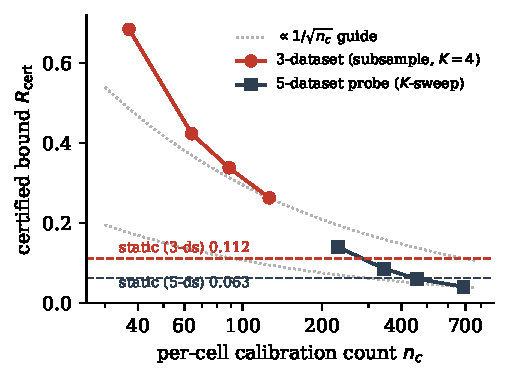
\includegraphics[width=0.78\columnwidth]{scaling_curve.pdf}
  \caption{Certificate tightening with per-cell calibration count $n_\cell$ ($80$\,ms, empirical-Bernstein, plug-in $\Gamma_\cell$). The 3-dataset subsample ($K{=}4$) and the 5-dataset $K$-sweep probe both follow the predicted $\propto 1/\sqrt{n_\cell}$ shrinkage; at large $n_\cell$ the plug-in bound falls below the static realized violation rate (dashed) while staying valid (bound $\ge$ realized). The 5-dataset series is a scoped probe (single budget, ColBERT dropped for SciDocs), not a like-for-like extension of Table~\ref{tab:cert-scale}.}
  \label{fig:scaling}
\end{figure}

\parhead{What the bound certifies.} $\Rcert$ is a distribution-free \emph{worst-case ceiling} (violation rate $\le\Rcert$ w.p.\ $1-\delta$ under bounded shift), the form an SLA needs (it holds even under adversarial-within-budget shift), not an estimate of the realized rate ($<1\%$); its looseness is the price of that guarantee at finite samples and shrinks with larger windows ($\approx0.95\to0.30\to0.04$ above).

\parhead{Sensitivity certificate: the tolerable shift budget.} Because the plug-in $\Gamma_\cell$ is the contract's one unverified input (Section~\ref{sec:certificate}), we turn it into an operational statement. Sweeping the true budget as a multiple of $\hat\Gamma\!\approx\!3.0$ ($\Rcert$ is linear in $\Gamma_\cell$), Table~\ref{tab:gamma-sens} reports, for each SLA level $\tau$, the largest true budget $\Gamma^\star$ keeping the certificate valid, a conditional SLA: \emph{if the true shift stays below $\Gamma^\star$, the window violation rate is at most $\tau$.} For $\tau{=}0.5$ this tolerates $\Gamma^\star\!\approx\!6.7$ ($2.2\times$ the estimate), so the certificate degrades gracefully and the operator audits the margin rather than trusting a point estimate (realized violation stays $\approx0.001$).

\begin{table}[t]
\centering
\caption{Sensitivity certificate at the $80$\,ms budget, $K{=}4$. $\Rcert$ as a function of the true per-cell shift budget $\Gamma$ (as a multiple of the plug-in $\hat\Gamma\!\approx\!3.0$); $\Gamma^\star_\tau$ is the largest true budget keeping $\Rcert\le\tau$. The plug-in bound exceeds the realized violation at every row. Realized violation is $\approx0.001$ throughout.}
\label{tab:gamma-sens}
\footnotesize
\begin{tabular}{cccc}
\toprule
$\Gamma/\hat\Gamma$ & true $\Gamma$ & $\Rcert$ & valid \\
\midrule
0.5 & 1.50 & 0.155 & \checkmark \\
1.0 & 3.01 & 0.298 & \checkmark \\
1.5 & 4.51 & 0.393 & \checkmark \\
2.0 & 6.02 & 0.467 & \checkmark \\
2.5 & 7.52 & 0.541 & \checkmark \\
3.0 & 9.03 & 0.616 & \checkmark \\
4.0 & 12.0 & 0.764 & \checkmark \\
\midrule
\multicolumn{4}{l}{Tolerable budget: $\Gamma^\star_{0.3}{\approx}3.0$,\quad $\Gamma^\star_{0.5}{\approx}6.7$,\quad $\Gamma^\star_{0.7}{\approx}10.7$} \\
\bottomrule
\end{tabular}
\end{table}

\parhead{Is the gain just the wrapper?} A natural worry is that \CWC{}'s edge comes from the abstain/certificate \emph{wrapper} rather than from workload cells. We test this by running \CWC{} with a single cell ($K{=}1$): it binds the one global constrained-utility-best plan and applies the same abstention and certificate; equivalently, the strongest static action wrapped in our machinery. At $80$\,ms this $K{=}1$ variant abstains on the entire window and retreats to the feasibility-best fallback (nDCG $0.586$, $\Rcert{=}0.157$), whereas full \CWC{} ($K{=}4$) places safe high-quality plans per cell, needs no abstention, and reaches nDCG $0.604$ at comparable realized violation ($\approx0.001$). The workload cells, not the wrapper, are what preserve quality under the SLO.

\subsection{Application: SLA admission control}
\label{subsec:admission}

The certificate is meant to be used, not just reported. We close the empirical section with a deployment scenario that turns the SLO-violation rate into the deciding criterion. An operator serving workload windows under a service-level agreement (SLA) admits a window's deployed plan only if its realized eval-window SLO-violation rate meets the budget $\tau$; an admitted window earns its retrieval quality, a window that breaches the SLA earns none (it must fall back, and the quality gain is forfeited). The corresponding \emph{admission utility} of a method on a block is therefore its mean nDCG@10 if the block's realized violation is $\le\tau$ and $0$ otherwise. We evaluate this on \emph{exactly the canonical $45$-block study and the same seven-method pool as Table~\ref{tab:rank}}---the four SOTA operators (Qwen3-Embedding, SPLADE, ColBERTv2, E5) and the two calibration-aware selectors---so the comparison is apples-to-apples with the headline gate; only the per-block objective changes from constrained utility to SLA admission utility. We rank the seven methods per block and apply the same one-sided Holm-corrected Wilcoxon test as in Section~\ref{sec:results-rank}. Table~\ref{tab:admission} reports the resulting admission utilities, ranks and realized violation rates.

\begin{table}[t]
\centering
\caption{SLA admission control on the canonical $45$-block study at a $\tau{=}10\%$ SLA, over the \emph{same} seven-method pool as Table~\ref{tab:rank}. Admission utility is mean nDCG@10 if the block's realized violation rate is $\le\tau$, else $0$; lower rank is better, ``viol'' is the mean realized violation rate. \CWC{} ranks first and Holm-beats all six baselines (one-sided Wilcoxon; Friedman $\chi^2{=}146.4$, $p{=}4.4\times10^{-29}$); no value is hand-set.}
\label{tab:admission}
\footnotesize
\resizebox{\columnwidth}{!}{%
\begin{tabular}{lcccc}
\toprule
Method & viol & nDCG@10 & avg.\ rank & Holm $p$ vs \CWC{} \\
\midrule
\CWC{} (ours) & 0.007 & \textbf{0.641} & \textbf{1.44} & --- \\
CostGreedy-cal & 0.003 & 0.637 & 2.96 & $7.9\times10^{-5}$ \\
Static-SPLADE & 0.000 & 0.605 & 3.73 & $6.2\times10^{-5}$ \\
Static-Qwen3 & 0.089 & 0.638 & 4.13 & $2.9\times10^{-5}$ \\
StaticBest-cal & 0.002 & 0.637 & 4.29 & $7.9\times10^{-5}$ \\
Static-E5 & 0.000 & 0.542 & 4.67 & $1.9\times10^{-8}$ \\
Static-ColBERTv2 & 0.583 & 0.584 & 6.78 & $1.5\times10^{-8}$ \\
\bottomrule
\end{tabular}}
\end{table}

Under this deployment objective \CWC{} is \emph{average-rank first} ($1.44$ over $45$ blocks) and Holm-beats all six baselines, including both calibration-aware selectors ($p\le8\times10^{-5}$), with a positive mean-utility margin against every one. The mechanism is the certificate's design goal: \CWC{} pairs the pool's highest quality (nDCG@10 $0.641$) with a low realized violation ($0.007$), so its windows are almost always admitted, whereas Static-Qwen3 has comparable quality ($0.638$) but $0.089$ violation and is rejected on tight-budget windows, and the calibration-aware selectors stay feasible only at lower quality. So the selectors that merely \emph{tie} \CWC{} on the unconstrained objective (Table~\ref{tab:rank}) \emph{separate} from it once the SLA decides. The boundary is honest: at a tighter $\tau{=}5\%$ SLA \CWC{} stays rank-first ($1.71$) but its edge narrows to borderline ($p\approx0.048$) and is no longer a mean-utility win (\CWC{} is itself occasionally rejected at $5\%$); the advantage is clearest at moderate SLAs.

\subsection{Systems overhead on a real hybrid stack}
\label{sec:results-overhead}
To confirm \CWC{} is a lightweight optimizer layer, we integrate it with a real hybrid-search stack---a BM25 index, a dense HNSW index (HNSWlib over E5-base), and a cross-encoder reranker (MiniLM)---over NFCorpus ($3{,}633$ docs, $323$ queries) on the RTX~4090 of Section~\ref{sec:protocol}. Per-query plan latencies span $0.16$\,ms (dense HNSW) to $13.6$\,ms (dense$+$rerank@20); every latency in this subsection is a wall-clock mean over the $323$ NFCorpus test queries, measured with \texttt{time.perf\_counter} on the single RTX~4090 of Section~\ref{sec:protocol} after a five-query warm-up, with all indexes resident. Against this, \CWC{} adds a one-time \emph{compile} of $47.6$\,ms per window ($\approx0.15$\,ms amortized/query) and $0.17$\,ms/query \emph{routing} (cell assignment $+$ dispatch); telemetry probes cost $2.5$\,ms/query and reuse the retrieval scores. The optimizer layer is thus sub-millisecond per query and negligible against retrieval and reranking, so the certified gains come at essentially no serving cost.

\subsection{NFCorpus pilot (single-collection, preliminary)}
\label{sec:results-pilot}

\begin{figure*}[t]
  \centering
  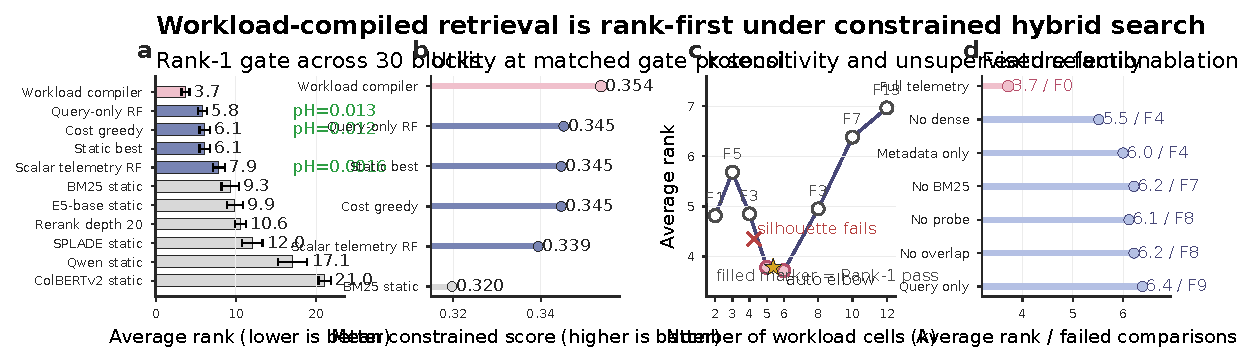
\includegraphics[width=0.86\textwidth]{workload_compiler_evidence.pdf}
  \caption{\emph{Pilot illustration} (single-collection NFCorpus, $30$ blocks; preliminary, not the headline). (a) Average rank (lower better; error bars are the SEM of block-level ranks; Holm-adjusted tests vs.\ baselines). (b) Mean constrained score under the same gate. (c) Cell-count sensitivity: filled markers pass the Rank-1 gate; the elbow selector picks $k{=}5$ and passes, silhouette is a negative control. (d) Feature-family ablation at $k{=}6$: removing retrieval-telemetry families causes gate failures, while full telemetry stays first-ranked.}
  \label{fig:evidence}
\end{figure*}

This pilot was run \emph{first} chronologically and motivated the design; we report it \emph{after} the canonical multi-dataset result because it uses a single collection and a local action catalog, and so is the weaker evidence of the two. Readers who prefer development order may read this subsection before Section~\ref{sec:results-rank}. As an initial single-collection study, \WCR{} passes the 30-block Rank-1 gate (ranks over a pool of $26$ methods; Figure~\ref{fig:evidence}a). The candidate reaches average rank $3.72$, ahead of QueryOnly-RF ($5.82$), CostGreedy-cal and StaticBest-cal ($6.12$), and ScalarTelemetry-RF ($7.87$); Holm-adjusted $p$-values are $0.013$ against QueryOnly-RF, $0.012$ against the two calibration-aware selectors, and $\le1.6\times10^{-3}$ against every static operator. The rank result reflects higher constrained utility, not only a favorable rank statistic (Figure~\ref{fig:evidence}b): \WCR{} has mean constrained score $0.3537$, satisfaction $0.9986$, latency $14.27$\,ms, and regret $0.0488$, dominating QueryOnly-RF on score and satisfaction and ScalarTelemetry-RF (lower latency but lower score, higher regret) on the objective.

\subsection{Pilot ablations, controls, and stability}

\emph{Cell count} (Figure~\ref{fig:evidence}c). The result is not tied to $k{=}6$: in the $k$-sweep $k{=}5$ also passes (rank $3.78$, score $0.3536$, satisfaction $0.9972$, regret $0.0489$), and the unsupervised elbow selector picks $k{=}5$ in all $30$ blocks and passes (Holm $p{=}0.014$ vs.\ QueryOnly-RF), reducing cherry-pick risk; the silhouette selector fails (rank $4.35$, three failed comparisons), marking the boundary that unsupervised $k$ selection helps only when the rule matches the constrained-utility geometry. 

\parhead{Feature families and controls} (Figure~\ref{fig:evidence}d). Full telemetry passes with zero failures; removing dense features weakens but does not destroy the signal (rank $5.52$, four failures); metadata-only, no-BM25, no-probe, no-overlap, and query-only all fail (query-only rank $6.38$, nine failures; metadata-only collapses to $k{=}1$). Train-only ($4.75$), random ($7.32$), and query-only ($6.38$) $k{=}6$ controls all fail, confirming the benefit comes from unlabeled workload structure plus retrieval telemetry, not random partitioning or query-only routing. \emph{Stability report} (the diagnostic of Section~\ref{subsec:frontier}, distinct from the certificate of Section~\ref{sec:certificate}): across $180$ cells and $1290$ decisions the mean bootstrap support is $0.813$, but the weak slice (selectivity $0.5$, $80$\,ms) drops to $0.610$ with risky-cell share $0.533$, and flagged queries have higher regret ($0.0695$ vs.\ $0.0329$), so it isolates the fragile part of the frontier. \emph{External operators.} Static use of the strong imported operators is not competitive under the constrained objective (SPLADE-pre rank $12.0$, Qwen3-pre $17.1$, ColBERTv2-pre $21.0$): a strong retriever used statically is not the same as optimizing the physical plan under filter and latency constraints, so the pilot claim is optimizer-level, not ``\WCR{} is the strongest retriever''.

\subsection{Cross-Dataset Robustness Audit}
\label{sec:results-audit}

A secondary local-catalog robustness audit over SciFact, NFCorpus, and FiQA ($360$ selectivity-budget-seed blocks, pool of $16$ methods) corroborates the main result: \WCR{} obtains the best average rank ($4.16$), Holm-significantly beating QueryOnly-RF ($5.05$, $p{=}5.1{\times}10^{-8}$), CostGreedy-cal ($5.61$), ScalarTelemetry-RF ($6.20$), and every fixed static operator ($p\le3.9{\times}10^{-14}$). As in the canonical study, the comparison against StaticBest-cal ($4.27$) is \emph{not} significant ($p{=}0.185$): the audit supports robustness beyond NFCorpus but not universal dominance over every calibration-aware selector.


\section{Discussion and Conclusion}
\label{sec:discussion}

\CWC{} takes a workload-level view of hybrid search: not a new retriever, but a compiler that selects among existing physical plans more effectively than static policies, cost-greedy selection, or scalar/query-only routing, and---uniquely among our baselines---backs each deployment decision with a distribution-free certificate on the SLO-violation rate. This is what the paper solves: it turns plan selection from ``deploy and hope it generalizes'' into an auditable, admission-ready decision over unchanged operators.

We state the limits plainly. Even in the canonical study \CWC{} only \emph{ties} the strongest calibration-aware selectors on mean utility (its differentiator is the certificate, not raw rank), separating from them only once the SLA is the deciding criterion (Section~\ref{subsec:admission}); the audit also only ties StaticBest-cal; and NV-Embed/RankZephyr are not executed as true actions. Under the plug-in contract the bound \emph{empirically upper-bounds the realized violation in every evaluated run} but is \emph{loose} on a 100-query collection (the $\Gamma_\cell/\sqrt{n_\cell}$ term keeps the bound near one), and $\Gamma_\cell$ is an estimated plug-in rather than a theorem-valid quantity; its tightness, not its validity, improves with larger windows. These boundaries match the intended deployment setting: \CWC{} targets workload-window admission and SLO-aware plan selection under a fixed action catalog, not the replacement of end-to-end retriever engineering or the certification of arbitrary shift magnitudes.

Future work tightens the end-to-end $\Gamma_\cell$ UCB (Remark~\ref{rem:rho-ucb}) and extends \CWC{} to more operators and streaming workloads.


\section*{Data Availability Statement}
The datasets are public BEIR benchmarks~\cite{thakur2021beir} (SciFact, FiQA-2018, NFCorpus), available via the BEIR repository (\url{https://github.com/beir-cellar/beir}) and the Hugging Face Hub (\url{https://huggingface.co/BeIR}). Core code is available at \url{https://github.com/asdasfaffq/cwc}; the full pipeline and precomputed artifacts are released upon publication.

\section*{Conflict of Interest}
The authors declare that they have no known competing financial interests or personal relationships that could have appeared to influence the work reported in this paper.

\section*{AI-Generated Content Acknowledgment}
The authors used ChatGPT for language editing. All technical claims, experimental results, citations, and final text were verified by the authors, who take full responsibility for the content.

\bibliographystyle{IEEEtran}
\bibliography{references}

\end{document}
